\section{Results and discussion}
\subsection{Optimalisation of the classifier parameters}
By performing a five fould crossvalidation during the trainingstage the most
optimal parameterset for the RF algorithm was searched for.  It was found that
for all levels except the first, a value of 5 yields optimal results for the
minimum samples per leaf parameter. For level 1, this optimal value was
significantly higher at 55. %TODO why? 
The accuray that was reached was respectively 80,5\%, 97,9\%, 98,1\% and 98,2\% for the
first, second, third and fourth level. This shows that the first two levels in
the cascade contributed more in the process of removing negative voxels the the
two last levels. The latter however were not useless as they still increased the
level of accuracy. The fourth level for example still eliminated about 600
voxels per scan.

For each level of the classifier a threshold was set to determine which voxels
would be allowed to the next level (i.e. which voxels showed a higher nodule
probability). In order to avoid discarding nodulevoxels of small nodules
a rather low threshold had to be set. These were empirically determined at 20\%,
40\%, 40\% and 70\% for the four levels respectively.

\subsection{Validation results}
%TODO inleiding images + images

The obtained sensitivity of the algorithm was 100\% with an average of 2,17 TP
per scan and an average of 4357 FP per scan. Training the algorithm on 30 scans
took 1 hour and 50 minutes. The processing of a new medium large dataset (136
slices) takes about 10 minutes.
% TODO FPs of FP?
Keeping in mind that comparing different studies is difficult (see
\ref{sec:performance}), some relevant results from literature are presented
here. \cite{teramoto} used a cylindrical nodule-enhancement filter and performed
a FP reduction using a SVM classifier. This method reached a sensitivity of 80\%
and 4,2 FP per LIDC/IDRI scan. The detection speed was 25-34 seconds per scan.
\cite{elbaz} applied template matching and found a sensitivity of 82,3\% and a
specificity of 9,2\%. The time to process 1 scan in C++ was about 5 minutes.
\cite{lee2010} tested an ensemble classification aided by clustering (CAC)
method on a set of nodules and non-nodule examples and they obtained a
classification accuracy of 97,72\%. An execution time of 190 seconds was
registered.

These results indicate our algorithm performed well concerning detecting all
nodules, but the amount of FP has to be reduced. The amount of FP can be reduced
in a first stage by determining the optimal value for each threshold.
Another way of improving the algorithm is increasing the amount of trainingdata.
To determine the optimal amount of datasets a comparison should be made between
the time it takes to train the algorithm on a certain amount of scans and the
improvements that are obtained in the performances of the algorithm by
increasing the amount of scans. A third possibility is implementing more
features (e.g. haar features), especially features focussing on removing edges
and eliminating the bronchioles. On the other hand, implementing more features
will increase the processing time. However, by optimising the thresholds in the
existing algorithm these things can also be (partially) achieved. The threshold
on level can be set higher which will remove more edges. For eliminating the
bronchioles the parameters of the 3D averaging features should be optimised. The
results from literature also show that we have a long processing time. However,
one has to take into account that the implementation of this algorithm was done
in Python -- an interpreted language -- which makes it inherently slower than
compiled languages such as C++. Nevertheless, Python was chosen for its rapid
prototyping abilities. Future work may implement our algorithm in C++ or another
compiled language to speed up the computational process.


\cite{ginneken} compared the performances of six nodule detection CAD algorithms
on the same validation dataset. The sensitivities at seven levels of false
positive detection were calculated and then averaged. The best performing method
in this study yielded an average sensitivity of 63,2\% for the detection of all
kinds of nodules. The sensitivity per nodule type was also provided: small
nodules (63,4\%), large nodules (62,8\%), isolated nodules (60,9\%), vascular
nodules (69,3\%), pleural nodules (43,5\%) and peri-fissural nodules (76,6\%).
This clearly shows that the ease of nodule detection also depends on the type of
nodule. As this information is not available in the annotations of the scans and
as we did not cooperate with a radiologist, it is not possible to differentiate
between the different types of nodules in this project. However, as we may
assume that different nodule types are represented in our testset, it is clear
the algorithm is able to detect several types of nodules except for extremely
small ones as we removed these from the annotations in the training and
validation phase.

\begin{figure}[ht]
\begin{center}
	\begin{subfigure}[b]{\linewidth}
		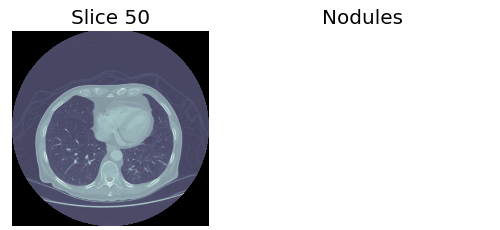
\includegraphics[width=\linewidth]{img/cascades/D50S50.png}
		\caption{Slice 50}
	\end{subfigure}
	\begin{subfigure}[b]{\linewidth}
		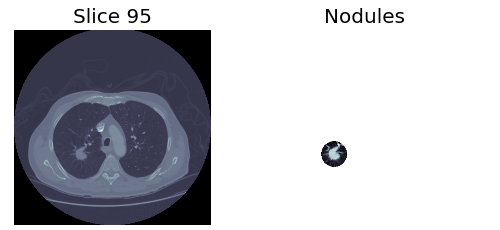
\includegraphics[width=\linewidth]{img/cascades/D50S95.png}
  		\caption{Slice 95}
	\end{subfigure}
	\caption{Example of two slices in dataset 50, one without and one with a
	nodule.}
	\label{fig:d50}
\end{center}
\end{figure}

\begin{figure*}[p] %TODO add percentage start/left, bigger threshold at end
\begin{center}
	\begin{subfigure}[b]{0.45\linewidth}
		\begin{subfigure}[b]{\linewidth}
			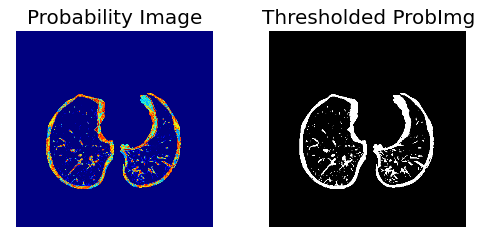
\includegraphics[width=\linewidth]{img/cascades/D50L1S50.png}
			\caption{Level 1 -- Threshold: xx\% -- xx\% remaining}
		\end{subfigure}
		\begin{subfigure}[b]{\linewidth}
			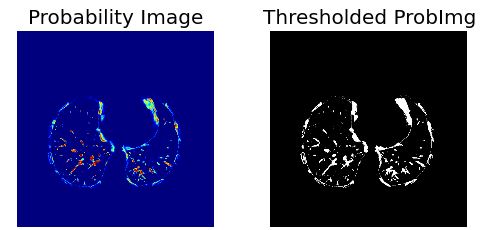
\includegraphics[width=\linewidth]{img/cascades/D50L2S50.png}
			\caption{Level 2 -- Threshold: xx\% -- xx\% remaining}
		\end{subfigure}
		\begin{subfigure}[b]{\linewidth}
			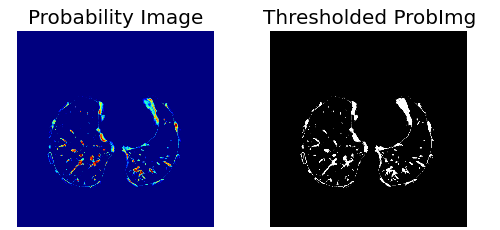
\includegraphics[width=\linewidth]{img/cascades/D50L3S50.png}
			\caption{Level 3 -- Threshold: xx\% -- xx\% remaining}
		\end{subfigure}
		\begin{subfigure}[b]{\linewidth}
			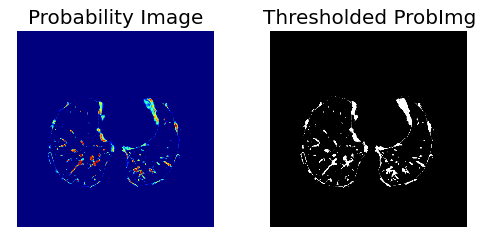
\includegraphics[width=\linewidth]{img/cascades/D50L4S50.png}
			\caption{Level 4 -- Threshold: xx\% -- xx\% remaining}
		\end{subfigure}
	  \caption{Processed versions of slice 50 in dataset 50. Left: probability
	  image. Right: threshold of probability image showing the voxels that continue
	  to the next level in the cascade.}
	  \label{fig:d50s50}
  \end{subfigure}
  \begin{subfigure}[b]{0.45\linewidth}
  		\begin{subfigure}[b]{\linewidth}
			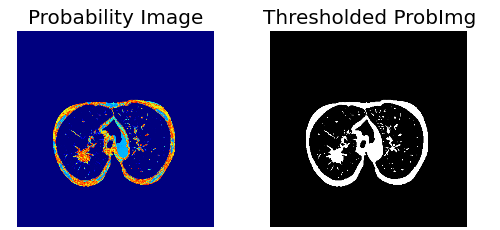
\includegraphics[width=\linewidth]{img/cascades/D50L1S95.png}
			\caption{Level 1}
		\end{subfigure}
		\begin{subfigure}[b]{\linewidth}
			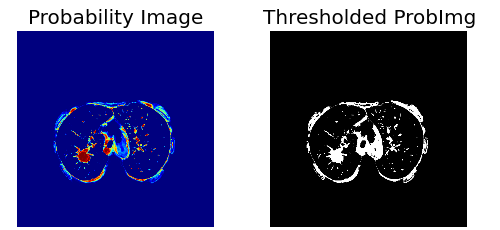
\includegraphics[width=\linewidth]{img/cascades/D50L2S95.png}
			\caption{Level 2}
		\end{subfigure}
		\begin{subfigure}[b]{\linewidth}
			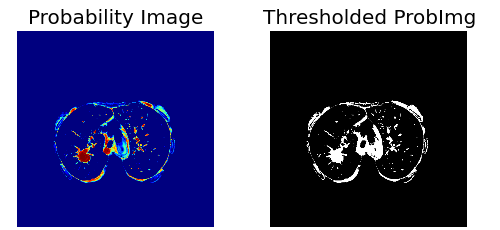
\includegraphics[width=\linewidth]{img/cascades/D50L3S95.png}
			\caption{Level 3}
		\end{subfigure}
		\begin{subfigure}[b]{\linewidth}
			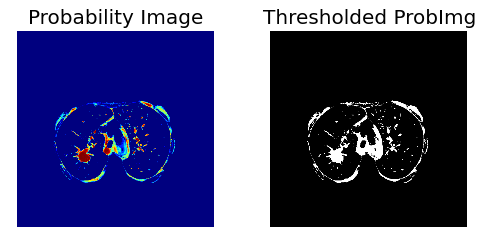
\includegraphics[width=\linewidth]{img/cascades/D50L4S95.png}
			\caption{Level 4}
		\end{subfigure}
	  \caption{Processed versions of slice 95 in dataset 50. Left: probability
	  image. Right: threshold of probability image showing the voxels that continue
	  to the next level in the cascade. The same thresholds and remaining counts
	  apply as in figure \ref{fig:d50s50}.}
	  \label{fig:d50s95}
  \end{subfigure}
\end{center}
\end{figure*}

% \begin{figure}[p]
% \begin{center}
% 	\begin{subfigure}[b]{\linewidth}
% 		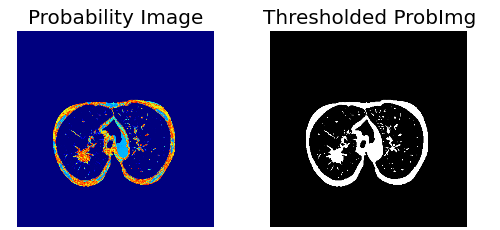
\includegraphics[width=\linewidth]{img/cascades/D50L1S95.png}
% 		\caption{Level 1}
% 	\end{subfigure}
% 	\begin{subfigure}[b]{\linewidth}
% 		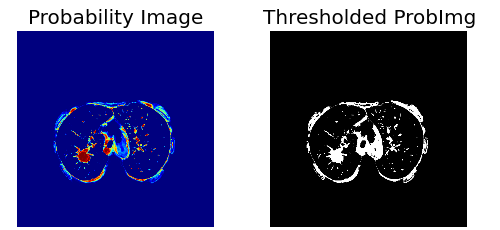
\includegraphics[width=\linewidth]{img/cascades/D50L2S95.png}
% 		\caption{Level 2}
% 	\end{subfigure}
% 	\begin{subfigure}[b]{\linewidth}
% 		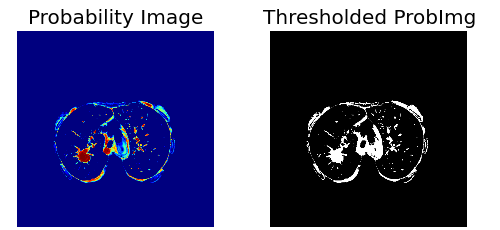
\includegraphics[width=\linewidth]{img/cascades/D50L3S95.png}
% 		\caption{Level 3}
% 	\end{subfigure}
% 	\begin{subfigure}[b]{\linewidth}
% 		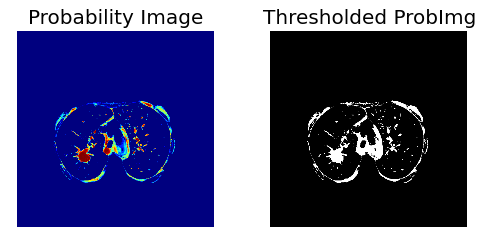
\includegraphics[width=\linewidth]{img/cascades/D50L4S95.png}
% 		\caption{Level 4}
% 	\end{subfigure}
%   \caption{Processed versions of slice 95 in dataset 50. Left: probability
%   image. Right: threshold of probability image showing the voxels that continue
%   to the next level in the cascade. The same thresholds and remaining counts
%   apply as in figure \ref{fig:d50s50}.}
%   \label{fig:d50s95}
% \end{center}
% \end{figure}